The general approach to the design of \pol{} protocols has been mainly focused on the proof generation process, as seen in the multiple examples dissected in Chapter~\ref{sec:related-work}. Advancements made towards more distributed and decentralized solutions have highlighted the need for a comprehensive and detailed description of the protocol's entire range of requirements. To achieve an operable system that meets the demands of real-world applications, a phased strategy with a keen awareness of the intrinsic details, at every stage of the solution, is essential for providing a complete and coherent picture of the protocol's design. The stages' interdependence may be later abstracted, either with a set of assumptions or a holistic approach, as argued later in this chapter, but the fact remains that the design of a \pol{} protocol starts with an infrastructural foundation, and ends with a complete system~\textemdash~aiming to achieve the goal of proving one's absolute location.

\begin{figure}[ht]
    \begin{center}
    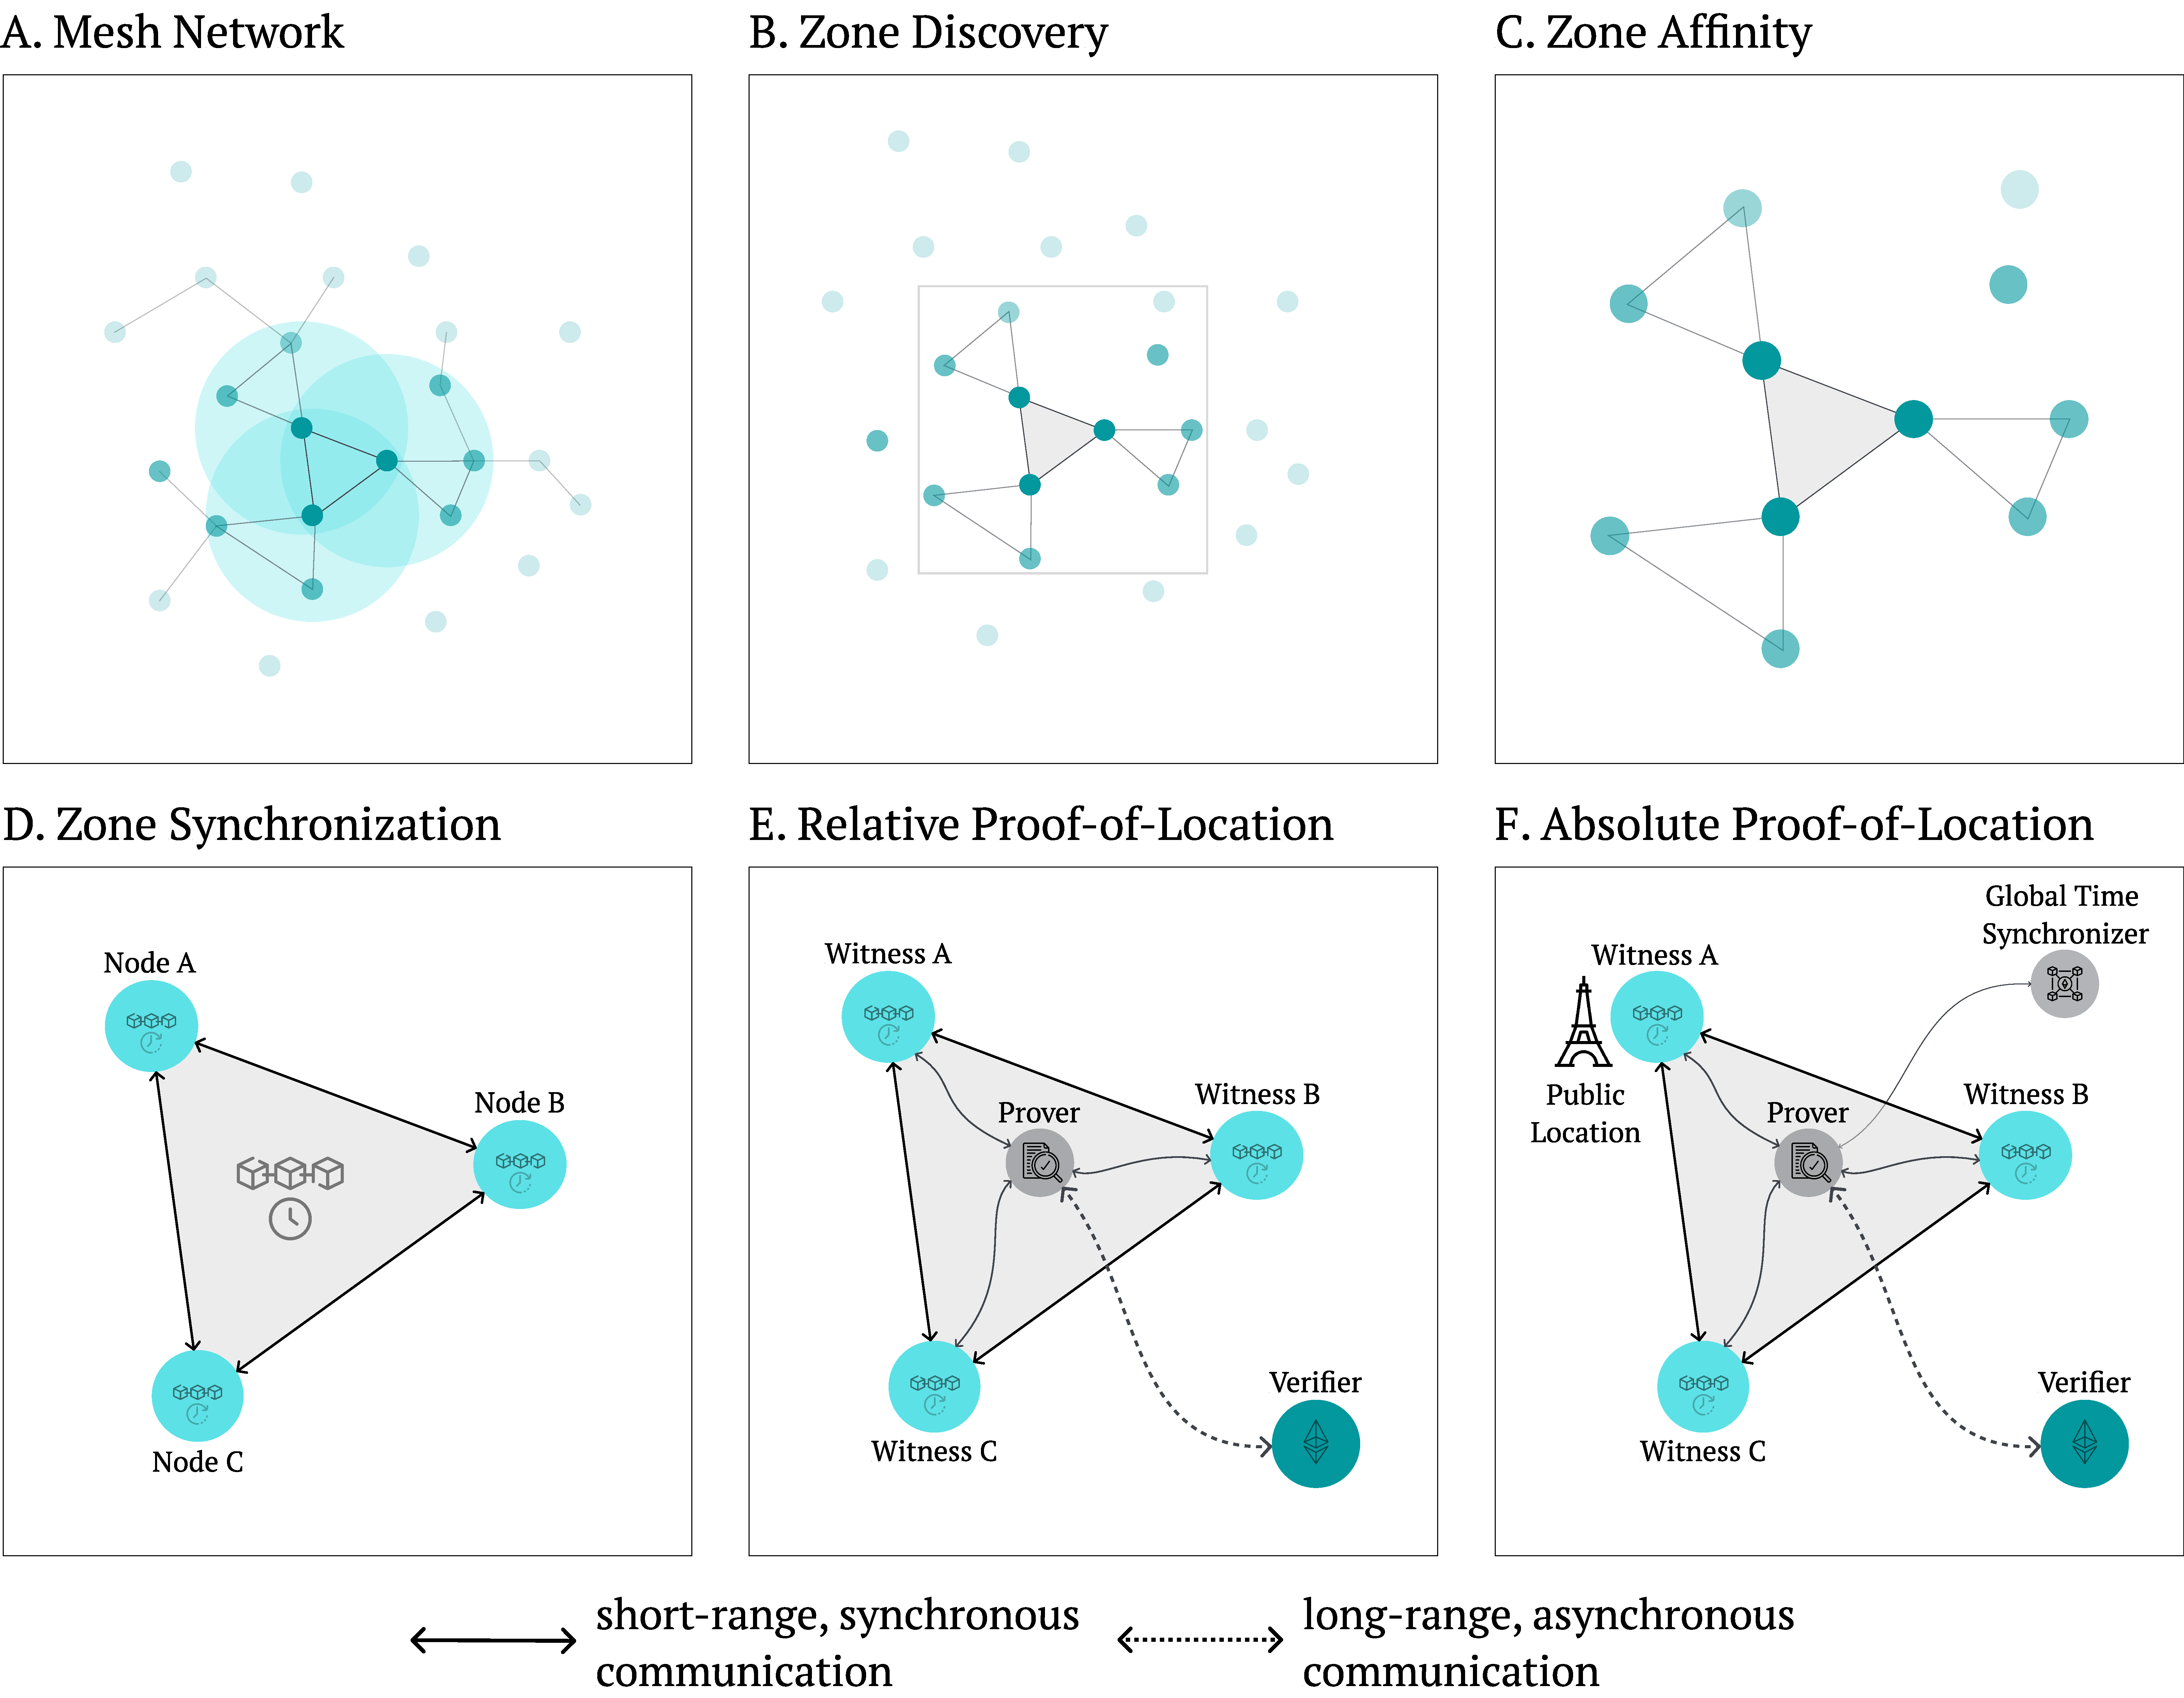
\includegraphics[width=0.9\textwidth]{overview-pol.pdf}
    \caption{A discretization attempt to capture the multiple steps of the protocol design overview, from a dynamic Mesh Topology, towards the ultimate goal of achieving Absolute \pol.}
    \label{fig:proof-of-location-overview}
    \end{center}
\end{figure}

The following sections will guide the reader through the multiple steps of the protocol's design. This design journey, depicted in Figure~\ref{fig:proof-of-location-overview}, starts with the understructure of the system, powered by a dynamic and non-hierarchic Mesh Network topology. This topology should enable the network agents to communicate with each other in a peer-to-peer, short-ranged, and conveniently wireless fashion. The next step entails the nodes' neighbourhood establishment, eased by lower-layer routing protocols, leading to the eventual creation of fully connected zones of neighbours. Each zone may abstractly form an individually bounded polygonal area, limited by its communication range. Each node, on the other hand, may simultaneously belong to multiple zones, with the processes of zone affinity, zone switching, zone expanding, and, consequently, the overall configuration of the mesh topology being dictated by protocolar arrangements, or even, application level incentives. The theoretical aim is at achieving a latticework of space and time, with zone-relative clock precision. Therefore, the next step is to establish, or derive, spatio-temporal zone synchronization. Space synchrony is achieved with the assumptions regarding the short-ranged communication means. Time synchrony requires a clock synchronization mechanism, which may simultaneously allow for zone-relative event serialization, via a Turing-complete strongly consistent consensus-based system. Nonetheless, the main aim is to achieve zone-relative time consciousness, to finally enable spatio-temporal soundness \cite{nasrulin2018robust}.

This thesis will provide, in the following sections, a more detailed analysis of these multiple steps, but will point only, in practical terms, to a subset of the entire problem. The steps that precede the zone discovery and zone affinity procedures, as well as the ones that succeed the goal of achieving relative \pol{} are either abstracted, explicitly assumed, or left for future work.

% \TODO{Should it be called "Zone Establishment"? Or rather "Zone Discovery"? Read the next section for more details... But keep this question in mind to decide what makes more sense}